\documentclass[]{article} 
\usepackage{pgfplots} 
\usepgfplotslibrary{external} 
\tikzexternalize 
\usepgfplotslibrary{fillbetween}
\usepackage{tikz} 
\usepackage{amsmath} 
\usepackage{pgfplots} 
\usetikzlibrary{calc} 
\pgfplotsset{compat = newest, every axis plot post/.style={line join=round}, label style={font=\Large},every tick label/.append style={font=\large}  }
\begin{document} 
	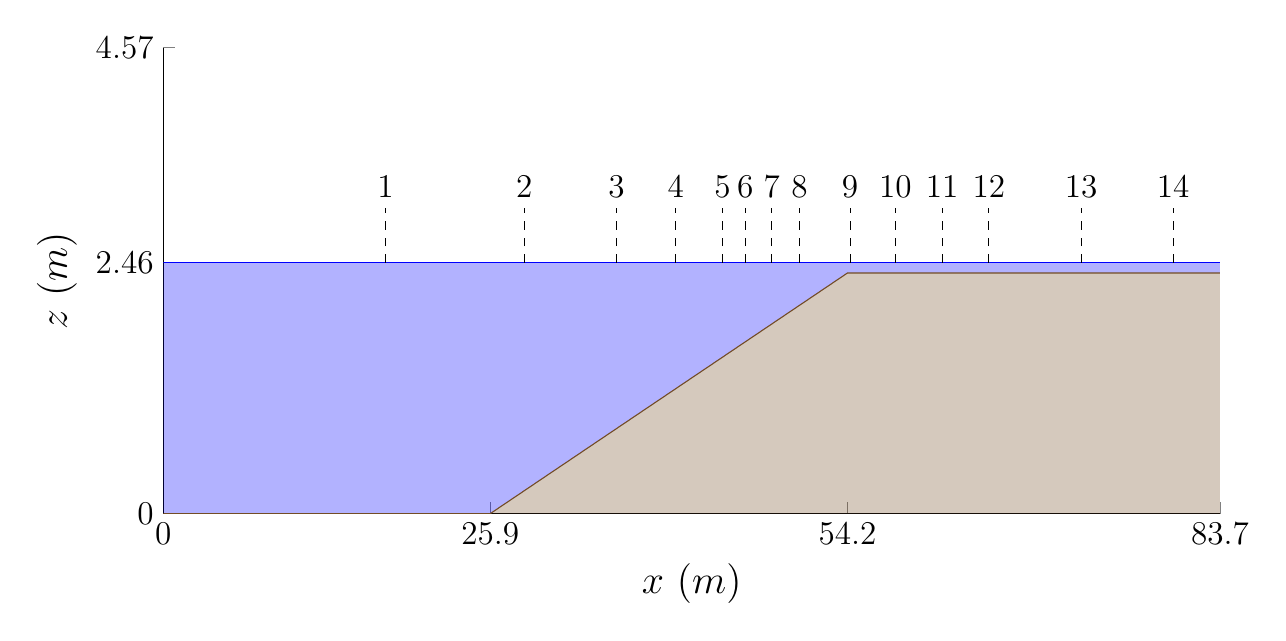
\begin{tikzpicture}
	\begin{axis}[ 
	width = 0.7\textwidth,
	width=15cm,
	height = 7.5cm,
	axis y line*=left,
	axis x line*=bottom, 
	xtick={0,25.9,54.2,83.7},  
	ytick = {0,2.46,4.57}, 
	xmin=0, 
	xmax=83.7, 
	ymin =0, 
	ymax = 4.57,
	xlabel=$x$ ($m$), 
	ylabel=$z$ ($m$)]
	
	\addplot [name path=b,brown!60!black] coordinates {(0,0) (25.9,0) (54.2,2.36)  (83.7,2.36)};
	
	\path[name path=axis] (axis cs:0,0) -- (axis cs:83.7,0);
	
	\addplot [name path=a,blue] coordinates {(0,2.46) (83.7,2.46)};
	
		\addplot [
		thick,
		color=brown!60!black,
		fill=brown!60!black, 
		fill opacity=0.3
		] fill between[of=b and axis];
		
	\addplot [
	thick,
	color=blue,
	fill=blue, 
	fill opacity=0.3
	] fill between[of=a and b];
	
	
	\addplot [black,dashed] coordinates {(17.6,2.46) (17.6,3)};
	\node[above] at (axis cs:17.6,3) {\large$1$};
	\addplot [black,dashed] coordinates {(28.6,2.46) (28.6,3)};
	\node[above] at (axis cs:28.6,3) {\large$2$};
	\addplot [black,dashed] coordinates {(35.9,2.46) (35.9,3)};
	\node[above] at (axis cs:35.9,3) {\large$3$};
	\addplot [black,dashed] coordinates {(40.6,2.46) (40.6,3)};
	\node[above] at (axis cs:40.6,3) {\large$4$};
	\addplot [black,dashed] coordinates {(44.3,2.46) (44.3,3)};
	\node[above] at (axis cs:44.3,3) {\large$5$};
	\addplot [black,dashed] coordinates {(46.1,2.46) (46.1,3)};
	\node[above] at (axis cs:46.1,3) {\large$6$};
	\addplot [black,dashed] coordinates {(48.2,2.46) (48.2,3)};
	\node[above] at (axis cs:48.2,3) {\large$7$};
	\addplot [black,dashed] coordinates {(50.4,2.46) (50.4,3)};
	\node[above] at (axis cs:50.4,3) {\large$8$};
	\addplot [black,dashed] coordinates {(54.4,2.46) (54.4,3)};
	\node[above] at (axis cs:54.4,3) {\large$9$};
	\addplot [black,dashed] coordinates {(58.0,2.46) (58.0,3)};
	\node[above] at (axis cs:58.0,3) {\large$10$};
	\addplot [black,dashed] coordinates {(61.7,2.46) (61.7,3)};
	\node[above] at (axis cs:61.7,3) {\large$11$};
	\addplot [black,dashed] coordinates {(65.4,2.46) (65.4,3)};
	\node[above] at (axis cs:65.4,3) {\large$12$};
	\addplot [black,dashed] coordinates {(72.7,2.46) (72.7,3)};
	\node[above] at (axis cs:72.7,3) {\large$13$};
	\addplot [black,dashed] coordinates {(80.0,2.46) (80.0,3)};
	\node[above] at (axis cs:80.0,3) {\large$14$};

	\end{axis} 
	
	
	
	\end{tikzpicture}
\end{document}